% id: 120-08
% book: 100발100중 3-2 기말 · 01 3-2 기말(원의 성질·통계·부록)
% section: 고난도 기출문제
% figure: crop:fig-120-08.png
% answer: ②
% answer_source: 답지(빠른정답)
% variant_level: 0 (원본 전사)
% 이 파일은 build.mjs 가 items.json 에서 만든다. 고칠 때는 items.json 을 고친다.
\smash{\raisebox{1.5mm}{\dmkichul{100발100중 3-2 기말 120쪽 08번}}}
\noindent\begin{minipage}[t]{0.58\linewidth}\vspace{0pt}\raggedright 그림에서 $\overrightarrow{\pt{PQ}}$와 $\overrightarrow{\pt{PR}}$는 원~$\pt{O}$의 접선이고, 점~$\pt{B}$와 점~$\pt{C}$는 접점이다. $\angle\pt{ABO}=30^\circ$, $\angle\pt{ACR}=68^\circ$일 때, $\angle\pt{BPC}$의 크기는?\end{minipage}\hfill\begin{minipage}[t]{0.4\linewidth}\vspace{0pt}\centering 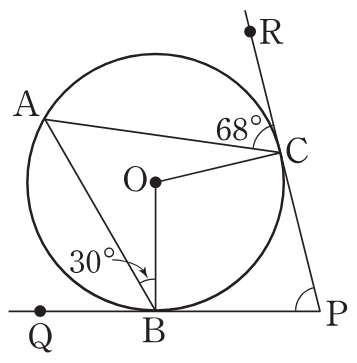
\includegraphics[width=85.6pt]{figures/fig-120-08.png}\end{minipage}\par
\begin{choicesii}{$74^\circ$}{$76^\circ$}{$78^\circ$}{$80^\circ$}{$82^\circ$}\end{choicesii}
